\chapter{Methodology}
	The specific implemented approach to find solutions for equation \ref{eq:problem} is explained
	in detail in this chapter. Important components of the solution described here include the
	modeling of the hyperparameter space and its sampling, the choice of the numerical optimization
	method, and the definition of the target function to optimize, among others.

	The general strategy followed here is summarized in figure \ref{fig:generalapproach}:

	\begin{figure}[here]
		\begin{center}
			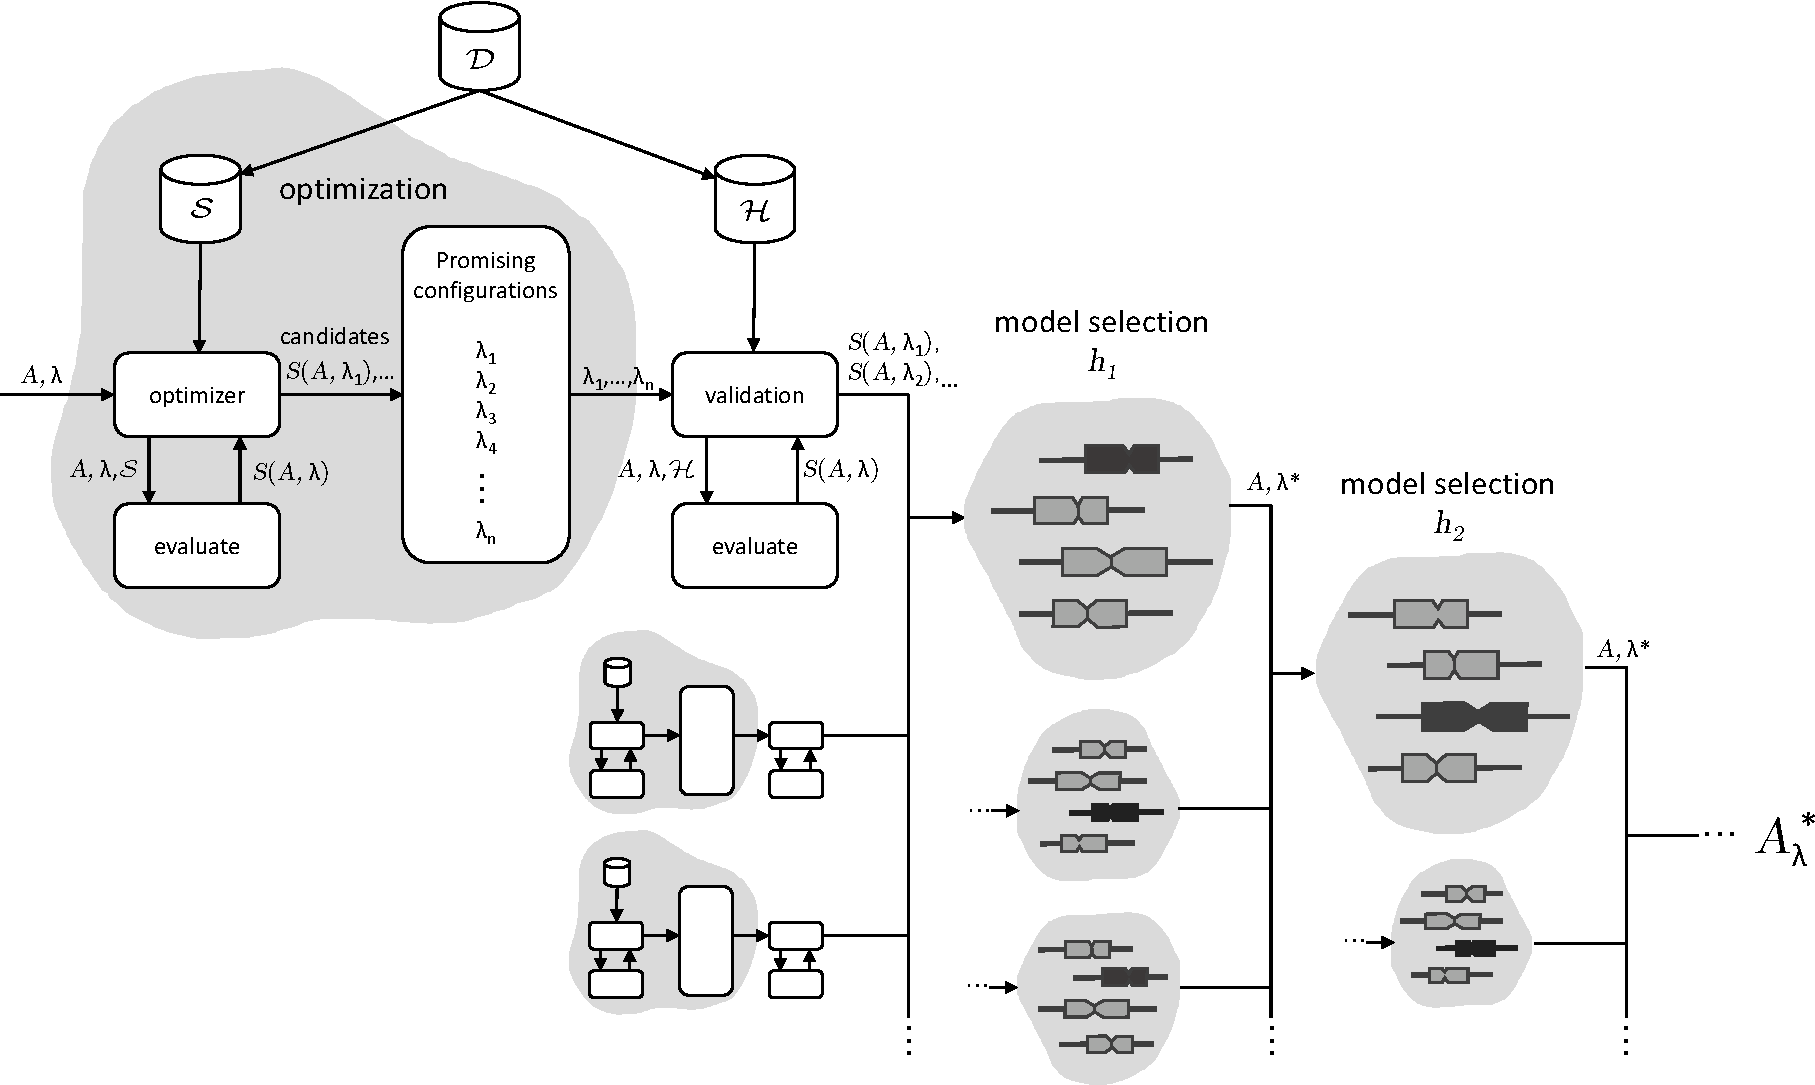
\includegraphics[width=\textwidth]{optimization_and_model_selection}
		\end{center}
		\caption[General methodology diagram]{Interaction between different components of the
		implemented hyperparameter optimization and model selection approach.}
		\label{fig:generalapproach}
	\end{figure}


	The entire process is subdivided in two stages. The instances contained in the dataset
	$\alldata$ are divided into two subsets $\selectionset$ and $\holdoutset$. The {\bf
	hyperparameter optimization stage} evaluates a large number of models (SML algorithm under a
	given configuration) on the subset $\selectionset$, in order to find the ones that exhibit the best
	predictive performance. The {\bf model selection stage} analyzes the selected models obtained
	from the hyperparameter optimization stage (candidates) under the subset $\holdoutset$ (data unseen to the
	optimization process), to assess
	generalization, and uses that information, along with other desirable properties of the models,
	to systematically rule out suboptimal models and finally return the best.


\section{Hyperparameter space modeling}
	\label{sec:hyperparam_dist}
	Most SML algorithms contain configuration options that control different aspects of their
	internal behavior, which can be further adjusted to fit specific needs. For example, algorithms
	that make use of the distance between examples in feature space might accept a distance metric
	to be specified, or algorithms that internally create trees might allow the user to specify a
	branching factor (maximum number of branches per node), and so on. Since SML algorithms accept
	a set of example instances for training and unseen data for predicton as \emph{parameters} 
	(equation \ref{eq:sml_alg}), and since the configuration options control the behavior of the
	algorithm, they are regarded to as \emph{hyperparameters} of the SML algorithm. The choice of
	hyperparameter values for a SML algorithm can heavily impact its predictive power.

	Different types of hyperparameters exist. Nominal hyperparameters take values from a fixed
	list of categories that usually correspond to a decision of \emph{how} the SML algorithm
	performs the predictions. Such {\bf categorical hyperparameters} include, for instance, which
	kernel to use to compute support vectors in a support vector machine classifier, or whether to
	consider the distance between neighboring points or not on the prediction of a k-nearest
	neighbors classifier. Once all these decisions have been made, {\bf numerical hyperparameters}
	control the values to use for the specific implementation of internal formulas needed for
	prediction, such as the number of neighbors for k-neighbors classification, or the cost
	parameter used by a support vector machine as a trade-off between allowing training errors and
	fitting the support vectors to the training set rigidly.

	Other considerations such as restricting the value of a numerical hyperparameter to a fixed
	range (addressed here by assigning validation rules for each numerical hyperparameter), or
	encoding dependencies between categorical and numerical or other categorical hyperparameters
	(implemented here as explained in detail in subsection \ref{ssec:hyp_hierarchy}) must be taken
	into account when modeling the strategy to explore the hyperparameters of a SML algorithm.

	\subsection{Hyperparameter distributions}
	\label{ssec:hyperparam_dist}
	Since one of the main objectives of this work is to learn the behavior of SML algorithms under
	different settings, a systematic way of obtaining valid candidate configurations for performance
	evaluation is required. In order to achieve this, each hyperparameter is regarded as a random
	variable and a distribution for its specific type is assigned to it.

	A one-dimensional distribution is used to sample values for each hyperparameter
	independently. Section \ref{ssec:hyp_hierarchy} describes in detail how dependencies between
	hyperparameters are handled. Drawing values for a hyperparameter from a distribution (other than
	a Uniform one) will favor some regions of the hyperparameter space over others, which can be
	useful when there is a good knowledge of what values for the hyperparameter produce good
	predictions.  It is possible that the choice of specific values for the \emph{categorical}
	hyperparameters affects what values for a numerical hyperparameter yield good results. Because
	of this, the same numerical hyperparameter is modeled with different distributions for different
	combinations of the categorical hyperparameters.

	\begin{figure}[t]
		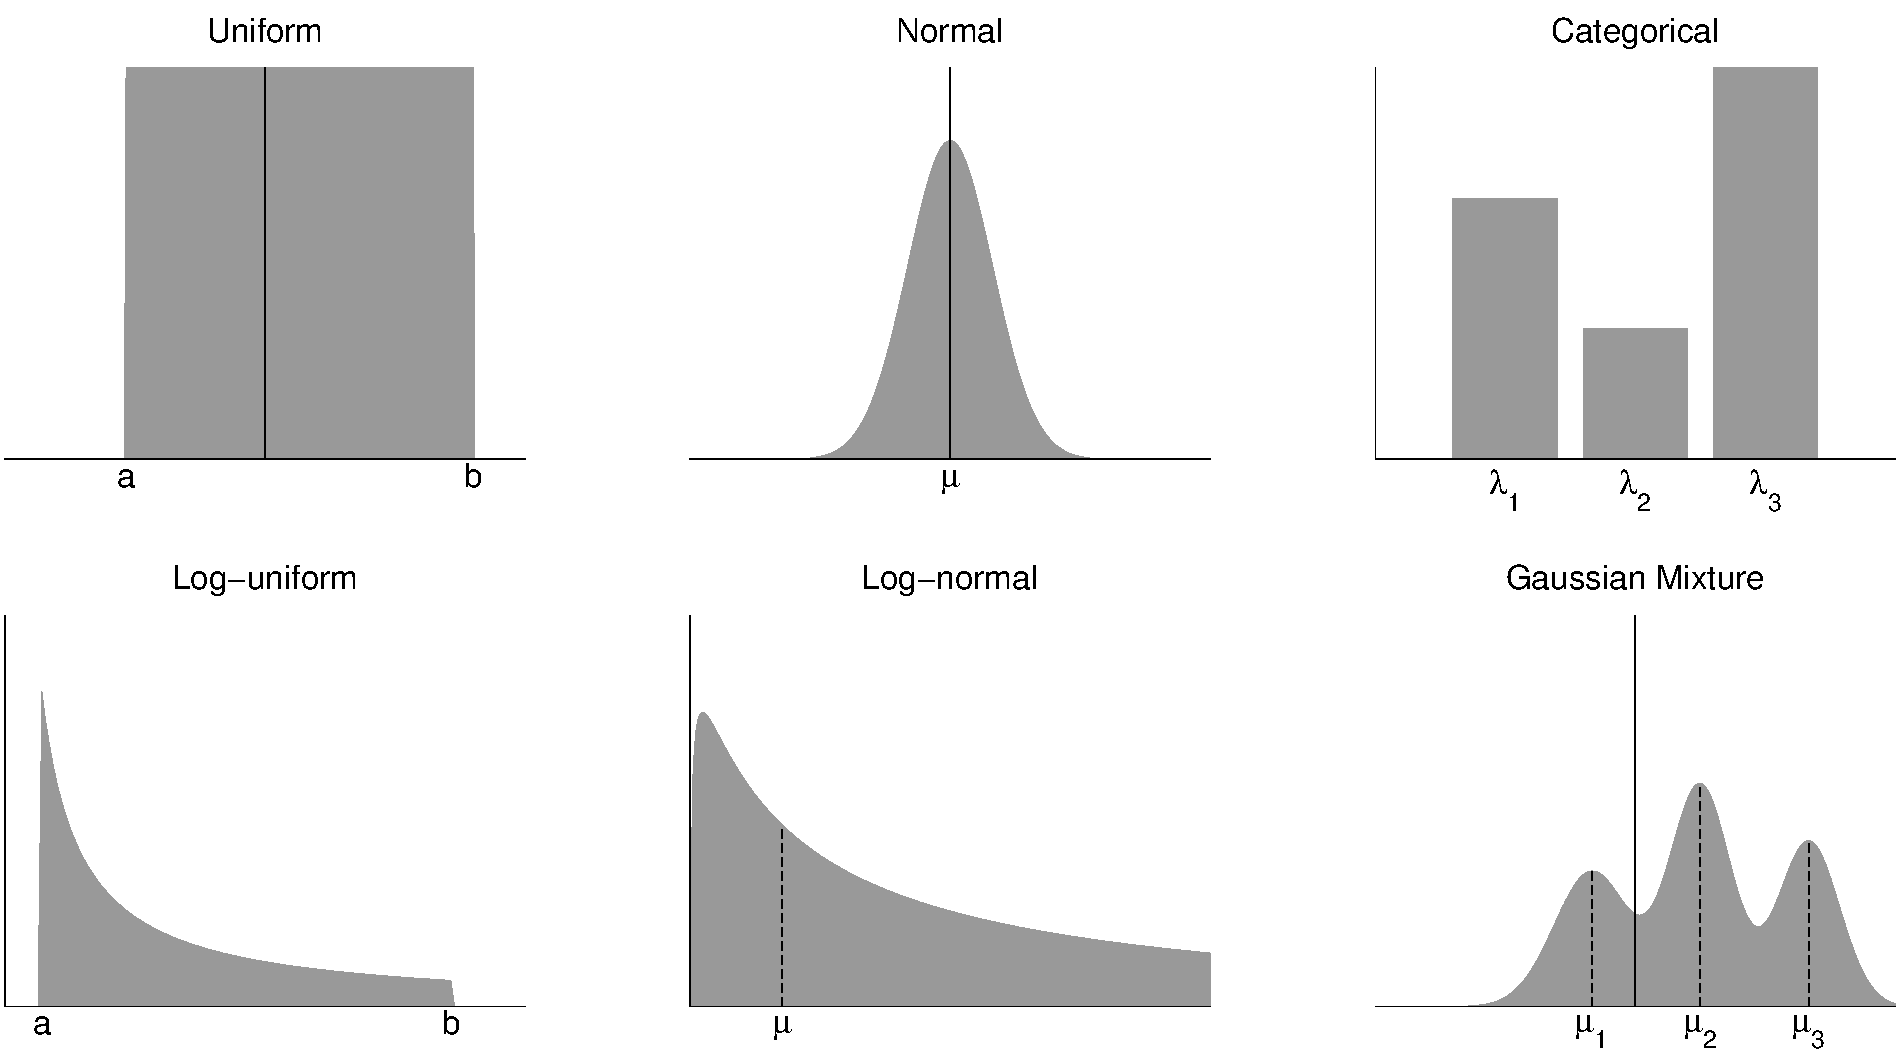
\includegraphics[width=\textwidth]{fig_dist}
		\caption{Distributions used to model hyperparameters}
		\label{img:distributions}
	\end{figure}

	The choice of the distribution depends on the nature of each hyperparameter and the knowledge of the
	range and expected values that the hyperparameter might take. The implemented types of prior
	distributions, depicted in figure \ref{img:distributions}, are:
	\begin{itemize}
		\item {\bf Categorical} distributions assigned to hyperparameters that can take nominal values
		from a list of $k$ fixed categories, or to discrete numerical hyperparameters.
		\begin{align}
			p(x) &= p_1^{[x=1]}\cdot \ldots \cdot p_k^{[x=k]}, & x \in \{1,\ldots,k\}
		\end{align}
		($[x=i]$ is the \emph{Iverson bracket}: $[P] = 1$ if statement $P$ is true, $0$ otherwise)
		\item {\bf Uniform} distributions assigned to continuous numerical parameters within a
		bounded range $[a,b]$.
		\begin{align}
			p(x) &= \frac 1 {b - a}, & a \leq x \leq b
		\end{align}
		\item {\bf Normal} distributions assigned to continuous unbounded numerical parameters, when
		a specific value $\mu$ and mean variation $\sigma$ is expected.
		\begin{equation}
			p(x) = \frac 1 {\sigma \sqrt{2\pi}} e^ \frac {-(x - \mu)^2} {2 \sigma^2} =
			\mathcal{N}(\mu, \sigma)
		\end{equation}
		\item {\bf Log-uniform} distributions for hyperparameters that might span over different
		orders of magnitude.
		\begin{equation}
			p(x) = \frac 1 {x(\ln b - \ln a)}
		\end{equation}
		\item {\bf Log-normal} distributions assigned to hyperparameters that can not have negative
		values, and for which a specific value and variability is expected.
		\begin{equation}
			p(x) = \frac 1 {x\sqrt{2\pi}\sigma} e^ \frac{-(\ln x - \mu)^2} {2\sigma^2}
		\end{equation}
		\item {\bf Gaussian Mixture Models} (GMMs) are used for continuous hyperparameters that are
		known to be multimodal.
		\begin{align}
			p(x) &= \sum_{i=1}^N \pi_i \mathcal{N}(\mu_i, \sigma_i),&\sum_{i=1}^N \pi_i = 1
		\end{align}
		GMMs have many parameters and thus should be used when there is solid knowledge of the
		shape of the hyperparameter distribution. GMMs are learned by analyzing the
		distribution of each hyperparameter on a large number of datasets and infer promising and
		harmful regions of the hyperparameter space, as explained in detail in chapter
		\ref{ch:learn}. 
	\end{itemize}

	The values for the category weights, means, variances, and bounds, depend on how each specific
	hyperparameter is used by the SML algorithm. By default, handcrafted distributions have been designed
	led by interpretation of the documentation of each SML algorithm, but can be later modified. For
	instance, a hyperparameter that, according to the documentation, is used by the implementation
	of the SML algorithm as a ratio, will be assigned a Uniform(0,1) distribution by default, but if the
	documentation suggests that values around 0.5 often yield good results, a gaussian distribution
	centered at 0.5 is assigned instead. The parameters for all distributions for all
	hyperparameters are stored as plain text in a configuration file, and can be manually edited if
	desired.

	\subsection{Hyperparameter hierarchy}
	\label{ssec:hyp_hierarchy}
	For most SML algorithm implementations, choosing specific values for some hyperparameters may
	change which other hyperparameters are also used or ignored, and how they are used by the
	algorithm. For instance, the SVM family of algorithms can use linear,
	polynomial, sigmoid, or RBF kernels, and if a polynomial kernel is chosen, it is possible to
	specify its polynomial degree; such option has no effect when a linear kernel is used. Likewise,
	it is possible to specify the intependent term for the polynomial and sigmoid functions used as
	kernels, and such value may have a different impact and different extrema depending on which
	kernel they operate on. The popular SVM implementation libSVM accepts a single hyperparameter
	\texttt{coef0} for this setting. Disregarding the duality of this hyperparameter and its
	dependence on the context (selected kernel in this case) when modeling and optimizing it might
	lead to unwanted results.

	What the above example implies is that it is mandatory to consider each hyperparameter for
	optimization within a context given by the values of other hyperparameters (the {\bf
	hyperparameter context}). A hierarchical design is chosen, based on two observations:
	\begin{enumerate}
		\item
		Hyperparameter contexts can be nested. The use and semantics of a hyperparameter may depend
		on the value of other hyperparameters, which may in turn depend on others.
		\item
		The hyperparameter context is always defined by a set of \emph{categorical}, rather than
		numerical, hyperparameters. Since the decision of whether or not to use a hyperparameter is
		a discrete (boolean) value, it does not make sense to consider continuous numerical
		variables when defining a hyperparameter context.
		
		%In the rare cases that numerical hyperparameters might decide the fate of others, artificial
		%boolean categorical hyperparameters can be added trivially, used for the structured
		%sampling, and discarded before running the actual algorithm. These artificial hyperparameter
		%would hold the values (categories) True or False depending on the evaluation of rules applied on the numerical
		%hyperparameters.
	\end{enumerate}

	A specific situation where observation 2 may be violated is when a numerical hyperparameter depends
	on a \emph{rule} applied on another numerical hyperparameter, rather than on its actual value. For
	example, if hyperparameter $b$ is only used by the SML algorithm when hyperparameter $a$ adopts
	values within a given interval, and invalid otherwise. A \emph{virtual} hyperparameter
	\emph{$b$\_valid} with such rule (which would be a categorical hyperparameter with categories
	\{\emph{True}, \emph{False}\}) can be added to the hyperparameter hierarchy. Hyperparameter
	$b$ would exist in the hyperparameter context given by \emph{$b$\_valid=True} and would not
	exist in the hyperparameter context given by \emph{$b$\_valid=False}. Virtual hyperparameters
	are used only to guide the hierarchical hyperparameter sampling and validation, and should be
	removed from the configuration before passing it to the SML algorithm.

	The two observations indicated above allow to encode the entire hyperparameter space for a SML
	algorithm into a tree structure that models the hierarchical dependences between sets of
	hyperparameters. The top nodes of the tree refer to categorical hyperparameters that do not
	depend on the values of others, and each category creates a new hyperparameter context (branch)
	under which its depending categorical hyperparameters will be represented.
	
	The leaves of the tree correspond to the numerical hyperparameters that are valid for the
	deepest branching to which they belong. The branching of categorical hyperparameters corresponds to a
	series of decisions on what values the categorical hyperparameters take, and is refered to as
	the {\bf signature} of the numerical hyperparameter context. Figure \ref{fig:tree_example}
	provides an example of a hyperparameter hierarchy.
	\begin{figure}[here]
	{ \footnotesize
	\Tree[.DecisionTreeClassifier
		[.\fbox{criterion}
			[.Gini
				[ .\fbox{max\_features\_use\_preset}
					[.False
						[ .\tiny\rotatebox{90}{mfs~} ] [ .\tiny\rotatebox{90}{msd~} ] [ .\tiny\rotatebox{90}{md~} ] [
						.\tiny\rotatebox{90}{msl~} ]
					]
					[.True
						[ .\fbox{max\_features\_preset}
							[ .sqrt
								[ .\tiny\rotatebox{90}{msd~} ] [ .\tiny\rotatebox{90}{md~} ] [
								.\tiny\rotatebox{90}{msl~} ]
							]
							[ .log2
								[ .\tiny\rotatebox{90}{msd~} ] [ .\tiny\rotatebox{90}{md~} ] [
								.\tiny\rotatebox{90}{msl~} ]
							]
							[ .None
								[ .\tiny\rotatebox{90}{msd~} ] [ .\tiny\rotatebox{90}{md~} ] [
								.\tiny\rotatebox{90}{msl~} ]
							]
						]
					]
				]
			]
			[.Entropy
				[ .\fbox{max\_features\_use\_preset}
					[.False
						[ .\tiny\rotatebox{90}{mfs~} ] [ .\tiny\rotatebox{90}{msd~} ] [ .\tiny\rotatebox{90}{md~} ] [
						.\tiny\rotatebox{90}{msl~} ]
					]
					[.True
						[ .\fbox{max\_features\_preset}
							[ .sqrt
								[ .\tiny\rotatebox{90}{msd~} ] [ .\tiny\rotatebox{90}{md~} ] [
								.\tiny\rotatebox{90}{msl~} ]
							]
							[ .log2
								[ .\tiny\rotatebox{90}{msd~} ] [ .\tiny\rotatebox{90}{md~} ] [
								.\tiny\rotatebox{90}{msl~} ]
							]
							[ .None
								[ .\tiny\rotatebox{90}{msd~} ] [ .\tiny\rotatebox{90}{md~} ] [
								.\tiny\rotatebox{90}{msl~} ]
							]
						]
					]
				]
			]
		]]
	}

	\caption[Hyperparameter hierarchy example]{Hyperparameter hierarchy for a decision tree
	classifier. Numerical hyperparameters correspond to the leaves. Categorical hyperparameters
	(enclosed in a box) create branches for each category that they contain.}
	\label{fig:tree_example}
	\end{figure}

	The whole model selection process can be viewed as an extension of the hyperparameter hierarchy,
	where the set of all SML algorithms $\algoset$ to analyze corresponds to a categorical
	hyperparameter of the model selection. Each top-level branch contains the hierarchy (subtree)
	for all the different configurations for a specific type of algorithm (the {\bf algorithm
	family}).

	{\bf Note:} For simplicity, the solution has been designed under the assumption that numerical
	hyperparameters are independent of each other. Modeling dependences between numerical
	hyperparameters is outside the scope of this work, as it would require to model all the
	hyperparameters belonging to the same signature in the hierarchy as a single multidimensional
	distribution.

	\subsection{Sampling the hyperparameter space}
	\label{ssec:sampling}
	As stated in subsection \ref{ssec:hyperparam_dist}, a probability distribution models the
	parameter space of each hyperparameter, depending on their type and any prior knowledge
	available. These distributions are used by an optimization method to sample hyperparameter
	values and evaluate them.

	Recall that a SML algorithm accepts a configuration $\param = (\paramval_a, \paramval_b,
	\paramval_c, \ldots)$, i.e. a set of values or realizations of the hyperparameters $a$, $b$,
	$c$, \ldots. Sampling the hyperparameter space means obtaining such realizations by
	sampling the distributions describing each hyperparameter.

	Since all the information about the categorical dependencies is encoded into the tree structure,
	and numerical hyperparameters from the same context are assumed independent from each other, each
	numerical hyperparameter is sampled independently.
	
	Generating valid samples of the hyperparameter space of a SML algorithm reduces then to getting
	a valid signature (by recursively sampling the distributions of the categorical hyperparameters
	in the tree) and sampling each numerical hyperparameter in the context given by the signature
	independiently. The SML algorithm under the configuration resulting from joining all these
	values together is the \emph{model} to be evaluated over the data.

\section{Model performance measurement}
	\label{sec:performance_measurement}
	
	Once the strategy for generating models for evaluation has been established, the definition of a
	model performance metric is required. To measure the performance of a model means to quantify
	how well the prediction of it on unseen data is, and hence the quality of the labeling obtained
	on the prediction step of the model is the criterion to be measured.

	Because the performance measurements between different algorithms must be comparable, a method
	that is agnostic to the algorithm should be defined. The labeling returned by the prediction
	step of the model can be either a single class for each instance in the prediction set,
	or, for some classification algorithms, a vector describing the probabilities for each instance
	to be assigned to a specific class.
	
	Predictions consisting of specific classes are transformed into probability vectors with a value
	of 1 for the position corresponding to the assigned class, and 0 elsewhere. This step provides a
	consistent representation for the output of all classification algorithms. For regression, the
	single (possibly multidimensional) predicted value is used without further transformation.

	Many metrics comparing the expected and the predicted classes exist, and different metrics
	allow for evaluation of different properties of the prediction. Table \ref{tb:metrics}
	summarizes some of the most widely used.

	\begin{table}[!ht]
		\centering
		\begingroup
		%\def\arraystretch{1.8}
		\begin{tabularx}{\textwidth}{| l c X |}
			\hline
			Metric & Formula & Description \\
			\hline
			\multicolumn{3}{|l|}{\bf Accuracy}\\
			& $

				\begin{aligned}
					\frac {\fp + \tn} {\fp + \fn + \tp + \tn}
				\end{aligned}$
				& Ratio of correctly labeled instances\\
				\hline
			\multicolumn{3}{|l|}{\bf $F_\beta$ score}\\
			& $
				\begin{aligned}
					\frac {(1+\beta^2) \tp} {1+\beta^2 \tp+\beta^2 \fn+\fp}
				\end{aligned}
			$ & Weighted average of precision and recall. $\beta$ is the relative importance of the
			recall with respect to the precision\\
			\hline
			\multicolumn{3}{|l|}{\bf Brier score}\\
			& $
				\begin{aligned}
				\frac 1 N \sum_{t=1}^N \sum_{i=1}^R(p_{ti} - o_{ti})^2
				\end{aligned}
			$ & Squared difference of probabilities returned by the prediction $p_{ti}$ and true
			probabilities of the labeling $o_{ti}$.\\
			\hline
			\multicolumn{3}{|l|}{\bf Matthews correlation coefficient}\\
			& $
				\begin{aligned}
					\frac {\tp~\tn - \fp~\fn}
					{\sqrt{ (\tp + \fp)(\tp + \fn) (\tn + \fn) (\tn + \fn)}}
				\end{aligned}
			$ & Balanced measure of true and false positives and negatives, suitable for data
			having classes with very different frequencies.\\
			\hline
			\multicolumn{3}{|l|}{\bf Coefficient of determination (R$^2$)}\\
			& $
				\begin{aligned}
					1 -
					\frac{\sum_i (f_i - \bar{y})^2}
					{\sum_i (y_i-\bar{y})^2}
				\end{aligned}
			$ & Measure of fitness of the predictions to the expected classes.\\
			\hline
			\multicolumn{3}{|l|}{\bf Area under ROC curve}\\
			& $
				\begin{aligned}
					\int_{-\infty}^{\infty} TPR(y) P_0(y) dy
				\end{aligned}
			$ & Probability to obtain a better score with a randomly chosen correctly-classified
			instance than with a randomly chosen misclassified one.\\
			\hline
			%\multicolumn{3}{|l|}{\bf P-R curve}\\
			%& $
			%	\begin{aligned}
			%		formula
			%	\end{aligned}
			%$ & [description here]\\
			%\hline
			\multicolumn{3}{|l|}{\bf Mean absolute error}\\
			%{\bf Mean absolute error}
			& $
				\begin{aligned}
					\frac 1 n \sum_{i=1}^n |f_i - y_i|
				\end{aligned}
			$ & Absolute difference between predictions $f_i$ and true values $y_i$\\
			\hline
			\multicolumn{3}{|l|}{\bf Mean squared error}\\
			%{\bf Mean squared error}
			& $
				\begin{aligned}
					\frac 1 n \sum_{i=1}^n (f_i - y_i)^2
				\end{aligned}
			$ & Squared difference between predictions $f_i$ and true values $y_i$\\
			\hline
		\end{tabularx}
		\endgroup
		\caption[Components of the Performance Index]{Components of the Performance Index. $\tp$,
		$\tn$, $\fp$, and $\fn$ correspond to the \emph{true positive}, \emph{true negative},
		\emph{false positive}, and \emph{false negative} count, respectively. $P_0$ is the
		probability of an instance \emph{not} belonging to a class.}
		\label{tb:metrics}
	\end{table}

	Different metrics may adopt values from different ranges, and the interpretation of the
	actual values might also differ from metric to metric. As an example, the accuracy of a
	prediction is measured in the range between 0 and 1, and a \emph{greater} value means a better
	prediction. The mean squared error is measured as a positive value, and a \emph{lower} value means a
	better prediction in this case. In order to homogenize the metrics, upper and lower bounds are defined for
	each metric, and the relative position of the original value with respect to the bounded
	interval is used instead of the original value.

	The upper bound is straightforward to specify, as all metrics have an ideal value that would be
	achieved if the prediction agrees exactly with the true classes. To define the lower bound, the
	values for each of the metrics are calculated by using a virtual prediction that assigns the
	relative frequencies of each class in the dataset as the probabilities of any instance
	belonging to that class (this is equivalent to weighted-randomly assigning classes to the
	instances). The metrics obtained by this prediction are used as a {\bf baseline} that defines
	the lower bound of the interval for homogenization. It is possible that some homogenized metrics
	lie below the baseline, when the quality of the classification is worse than the baseline.

	The selected metrics are combined into a single {\bf performance index} to be used as the target
	function that the optimization method will aim to maximize. The performance index $\Score$ (also
	referred to as the {\bf \emph{score}}) is defined on a set of metrics $\allmetrics = \{m_1, m_2,
	\ldots, m_z\}$ as:
	\begin{align}
		\Score &= \sum_{i=1}^z w_i m_i(\expectedclasses, \predictedclasses), & \sum_{i=1}^z w_i = 1
		\label{eq:performance_index}
	\end{align}

	The weights $w_i$ control the relative importance of each metric and can be tuned to suit
	specific needs. For instance, if it is known that none of the SML algorithms to evaluate returns
	probability estimates of the labeling, the Brier scores will coincide with the reported
	accuracy, and is therefore safe to disable it by setting its weight to zero. All metrics are
	weighted uniformly by default.

	By default, the performance index used here combines the accuracy, the F$_\beta$ score, the
	Brier score, and the Matthews correlation coefficient. These metrics have some properties that
	make them suitable for a wide range of situations. The accuracy offers a very intuitive
	evaluation of the quality of the prediction, the F$_\beta$ score allows for tuning of the relative
	importance of the recall with respect to the precision, which might be useful depending on the
	needs of the user, the Brier score takes the probability estimates into account and therefore
	deals with ambiguity in the classification in a more fair way, the Matthews correlation
	coefficient is a balanced metric suitable for classes with very different relative frequency.

	While encoding metrics into a one-dimensional performance index may hide important details of
	the individual metrics, and yields values that are not straightforward to interpret, it is much
	more convenient to use it to represent the overall performance than dealing with a
	multidimensional score directly. The performance index described is thus the chosen approach for
	defining the optimization target function.

\section{Model validation}
Using a model validation protocol is important because it reduces the risk of overfitting a model to
the particularities of the training set, and hence is a first step to promote generalization of the
model to unseen data.
The performance index calculated by equation \ref{eq:performance_index} maps each model to a single
numerical value that represents its ability to correctly predict classes on a very specific set of training
and testing instances. In order to assess the predictive quality of the model in a more general
setup, repeated rounds of \emph{stratified $k$-fold cross-validation} are carried out. 

Each \emph{repetition} corresponds to a different random shuffling of the data. The $k$-fold
cross-validation splits the data into $k$ equally-sized portions (or folds), and uses one fold at a
time for prediction (and the remaining $k-1$ folds for training the model). \emph{Stratified} cross-validation
means here that the folds are enforced to all have the same proportion of examples for each class.

In most applications, a single repetition of 10-fold cross-validation is used, the scores obtained
for each fold are averaged out and used as a single score. This means that, for each fold,
the model is trained with 90\% of the data and tested against the remaining 10\%.
\cite{kohavi1995cv} justifies the choice of $k=10$ as the smallest number of folds with "acceptable"
bias. The actual number of repetitions and folds used in this work is exposed as a parameter that
can be customized at will.

For the optimization stage, the standard 10-fold cross-validation is used by default. For the model
selection stage, since a more limited number of candidate configurations will be evaluated, and
because a statistical analysis is to be performed on the distribution of results, a larger number of
evaluations for each model can and should be obtained. Normality of the distribution of scores is assumed.
Performing 3 repetitions of 10-fold cross-validation is suggested, to comply with the rule of thumb
of using a sample size of at least 30 samples to estimate a normal distribution.

\section{Optimization}

The optimization stage retrieves configurations, evaluates their performance, and uses the
performance measurements to guide the retrieval of new configurations towards regions of the
hyperparameter space expected to show predictive improvement.

Since the aim of this work is to provide the framework for hyperparameter optimization and model
selection, rather than to study different optimization techniques, only a couple of optimization
methods have been implemented. More sophisticated optimization methods such as simulated annealing
and genetic algorithms could also be used. The framework described here assumes only that the
optimization method returns candidate configurations, and can be fed with their evaluation results
in order to train itself if needed.

The valid optimization methods work on the numerical dimensions of the hyperparameter space
only. This is particularly convenient because most current optimization methods are purely
numerical, and the current design does not impose any further restrictions or special handling of
the non-numerical dimensions, which removes the need for specially designed optimization methods.

The optimization stage is restricted by a fixed time budget, shared across all the SML algorithms.

\subsection{Random search}

The easiest way to generate candidate configurations is to simply draw values at random for each
hyperparameter.

The considerations stated in  subsection \ref{ssec:sampling} must be respected, namely the
hyperparameter sampling must start from the root of the hyperparameter hierarchy, obtain a
realization of the top-level hyperparameter (randomly in this case), and use its value to decide
what other hyperparameters to sample. The categorical and numerical values retrieved are the
components of the configuration.

Random search does not need to keep track of the evaluated model history or the retrieved scores,
since every draw of hyperparameter values is independent of all the previous ones. As a consequence,
random search is a very slow and expensive optimization method. Random search is, however, very
useful when a more thorough exploration of the hyperparameter space is required, as it gives any
possible configuration the same chance to be drawn.

A very important application of random search is presented in chapter \ref{ch:learn}, where it is
used as a meta-optimizer for inferring hyperparameter distributions to train a parametric density
estimation optimizer.

\subsection{Shrinking hypercube}

Unlike the random search, the shrinking hypercube method described in \cite{Gonnet2010} does make
use of the scores returned by previous optimization rounds to guide the search to a local maximum.

The shrinking hypercube algorithm works by defining a region of the multidimensional parameter space
for exploration, delimited by a hypercube centered about the configuration that produces the best
result of all the tested configurations. The hypercube will shrink when no improvement is found, to
localize the search, and expanded when a new best is found, to stimulate exploration.

The pseudocode of the shrinking hypercube approach is presented in algorithm \ref{alg:shrink}

\begin{algorithm}[here]
	\begin{algorithmic}
		\State Sample and evaluate a random point from the numerical hyperparameter space.
		\State Define a hypercube of arbitrary length centered about the sampled point.
		\While {the size of the hypercube is larger than a threshold}
		\State Sample and evaluate another point randomly from within the hypercube.
		\If {the evaluation of the new point is better than the previous point}
			\State Duplicate the length of the hypercube on all dimensions.
			\State Center the hypercube about the new point.
		\Else
			\State Reduce the length of the hypercube on all dimensions by a small factor.
			\State Keep the hypercube centered about the current best point.
		\EndIf
		\EndWhile
	\end{algorithmic}
	\caption{Shrinking hypercube optimization}
	\label{alg:shrink}
\end{algorithm}

Duplicating the length of the hypercube on each dimension favors exploration of the
hyperparameter space since new configurations arbitrarily far from the current best can be reached.
Shrinking the hypercube slowly when no improvement is achieved helps localize the search for a local
maximum around the current best configuration while not significantly restricting the exploration.

The implementation used in this work considers each numerical hyperparameter space (each leaf in the
hyperparameter tree) as a single, independent hypercube, and finds local maxima for each one
independently. When the hypercubes are shrunk below a threshold, they are reset to a different
starting point and default hypercube side length. Multiple hypercubes can also be used
in parallel with different starting points and side lengths for a better coverage of the
hyperparameter space.

\subsection{Parametric density optimization}
A simple optimization approach that makes use of clues about generally high and low-scoring regions in the
hyperparameter space is presented in detail in chapter \ref{ch:learn}.

The distributions for all hyperparameters are estimated automatically, by running the optimization
process on a large set of standard datasets using random search to explore the hyperparameter space.
The results of all the datasets are used to fit gaussian mixtures that encode the high and
low-scoring regions for each hyperparameter. The gaussian mixtures returned by this process will replace
the default distributions that represent each hyperparameter.

\section{Model evaluation and selection}
The optimization stage explores the hyperparameter space and finds candidate configurations that
return a high performance index when evaluated on the \emph{optimization data set}. The selected
model will be chosen from one of such candidates according to their predictive performances on a
\emph{hold out dataset}, and other desirable criteria.

A very large number of candidate configurations might be proposed by the optimization process, and
hence a strategy to efficiently discard or promote configurations must be designed. 
The tree structure chosen to represent the hyperparameters of a SML algorithm can be exploited to
this end.

The chosen strategy analyzes the local optima found by the optimization process on the leaves of the
hyperparameter tree (which only contain numerical hyperparameters), selects the ones that are
significantly better, evaluates them and ranks them according to other desirable properties to
narrow down the model selection even further. When a handful of very good models are selected at the
numerical level, they are used to represent their branching in the tree at the deepest categorical
level, and compete with representative models of the other categories in the exact same way. The selected
models among all categories are promoted upwards to represent the category one level higher in the
hyperparameter tree. The process is repeated until the root branching of the tree is reached, i.e.,
when models from different SML algorithms are compared. A schematic of the process is shown in
figure \ref{img:tree}.

\begin{figure}[here]
	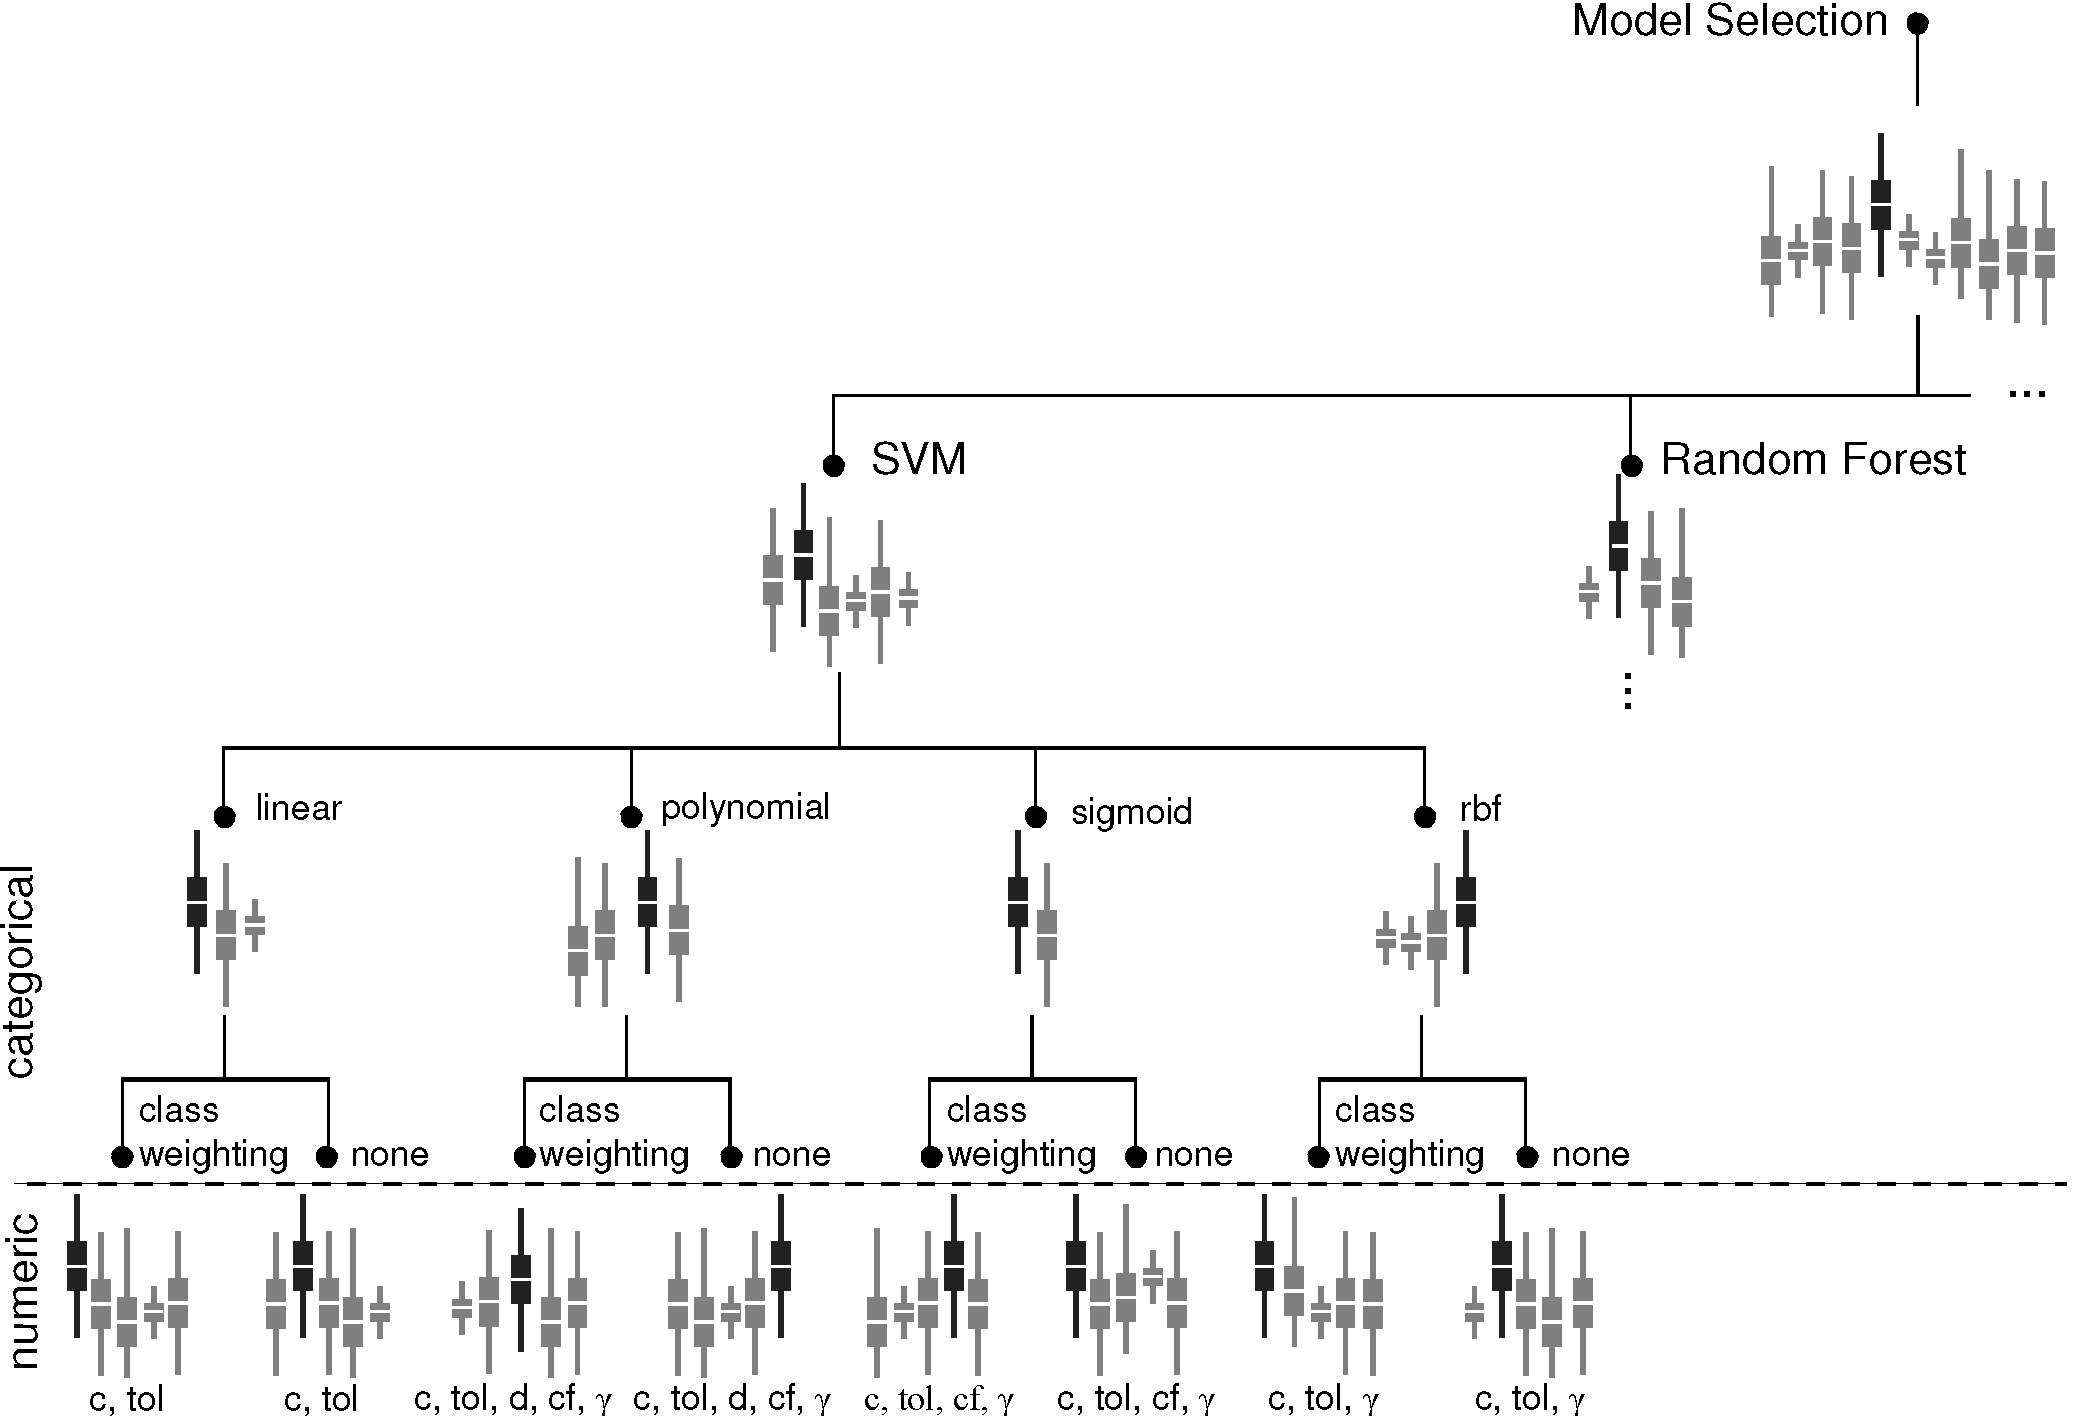
\includegraphics[width=\textwidth]{tree}
	\caption[Hierarchical model selection]{Hierarchical model selection. Each box plot represents
	the distribution of scores for a specific model. Distributions shown in black are promoted
	upwards to subsequently compete against models from the same local hierarchy.}
	\label{img:tree}
\end{figure}

\subsection{Candidate model filtering}
The optimization stage will mostly retrieve models with high performance indices. Most optimization
techniques try to find local optima, and as a consequence, they might end up testing a large number
of configurations close to each optimum. This means that the distribution of hyperparameter values
sampled and evaluated by the optimization stage will tend to have more density around the different
local maxima found. A clustering approach is used here to remove redundant configurations and only retrieve
high-scoring configurations from different local maxima. This avoids overrepresentation of
configurations from a single hill in the score landscape and returns a small number of
configurations that represent more homogeneously the regions that yield good scores.

Clustering the evaluated configurations with the {\bf $k$-means} algorithm is used here to retrieve
$k$ clusters of configurations, and choose the configuration with the highest score from each cluster as
one of the candidate configurations that will represent a specific numerical hyperparameter space.
The number of means has been arbitrarily chosen to $k = 10$ by default but can be modified via a
parameter setting if needed.

\subsection{Statistical analysis}

Given a set of models, the distribution of their scores on different versions of the hold out
dataset is studied to determine which model offers enough evidence to be considered the best one.

The hierarchical structure of the hyperparameter space groups models that share the same signature
together, at different levels. Statistical analysis is performed at all levels of the
hyperparameter space, starting from the configurations that differ only on their numerical
hyperparameters, and promoting good models to be compared to others at the immediately broader
level of aggregation (the category immediately above in the tree) repeatedly up to the highest level
in the hierarchy.

Each model is used for prediction on the hold out dataset several times by using $m$ repetitions of
$k$-fold cross-validation ($m=3,~k=10$ by default). A multiple comparison statistical test (MCT) is
applied on the distributions of $m\cdot k$ scores obtained for each model.

Parametric MCTs make use of direct measurements of the data (such as the mean and variance), whereas
non-parametric MCTs rely on comparisons of other properties of the data (e.g. the ranking of the
groups according to some criteria) which makes them more general and applicable to a wider range of
distributions, at the expense of statistical power \cite{sheskin2003statistics}. Parametric
comparison tests are more statistically powerful and are thus preferred over non-parametric
alternatives.  Parametric tests, however, are only valid under certain specific conditions, and when
such conditions are not met, non-parametric comparison tests must be used instead.

The MCTs determine, up to a certain probability $\alpha$, whether there are significant differences between a
group of distributions or not, but do not tell the actual distributions that show differences. A
\emph{post-hoc} test is required in order to find which distributions differ. Both parametric and
non-parametric post-hoc tests exist.

The aim of the statistical analysis in the context of this work is to compare the distributions of
performance indices for all candidate models with respect to the highest-scoring one, and discard
all the candidate models with strong statistical evidence that they perform worse. The models kept
are {\bf statistically indistinguishable} from the best one. The overall procedure is based on
\cite{pizarro2002mct} and \cite{demsar2006mct} for significance testing.

The chosen \emph{parametric} MCT is the {\bf one-way ANOVA test} \cite{fisher1925statistical}, which is a
generalization of the $t$-test that corrects for accumulated errors when performing comparisons
between more than two distributions, by comparing a statistic against a $F$-distribution that
considers the specific number of distributions to compare as a parameter.

The one-way ANOVA test can be used when:
\begin{enumerate}
	\item The observations for all the distributions are independent.
	\item The distributions are approximately normal. This is tested by applying the
	{\bf Kolmogorov-Smirnov test} (K-S test, validates that a sample comes from a given distribution) on
	the sample (after standardization) against a standard normal distribution $\mathcal{N}(0,1)$
	\item The distributions have homogeneous variances (homoscedasticity). This is tested by
	applying the {\bf Bartlett's test} \cite{bartlett1937} on the different distributions of scores.
\end{enumerate}

As stated above, a post-hoc test is required when the ANOVA test determines that there are
significant differences between groups of scores. The {\bf Tukey's honest significance test} compares
simultaneously all the groups of scores and informs what groups are significantly different. The
Tukey's test is then used to find the sets of performance indices that are not significantly
different from the the highest-scoring one. Here it is assumed safe to discard models that do not
pass the Tukey's test, and keep the rest for further analysis.

When the conditions to apply the parametric MCT are not met, the {\bf Kruskal-Wallis test} is
applied instead to decide if significant differences exist, and the {\bf Nemenyi test} is used as
the post-hoc test to find the actual significantly different groups in the same way as for the
parametric case.

All the statistical tests make use of a critical value to reject hypotheses with a level of
certainty $\alpha$. The choice of $\alpha$ for model selection affects what models are deemed
statistically indistinguishable from the best. A larger $\alpha$ will generally reject more models
than a smaller one. Since most of the models to compare may be very similar at the family level,
it is left up to the user to decide what $\alpha$ values to use, to manually control the number of
significantly indistinguishable models to select.

\subsection{Ranking criteria}
The statistical analysis reduces the number of candidate models to those that statistically perform
as good as the best, according to their performance indices. Other criteria are evaluated on the
selected models in order to compare them and decide which one is the best from a group of models
statistically indistinguishable from the best.

The criteria used here are described in table \ref{tab:ranking}. Each criterion is evaluated for each
candidate model, and used for ranking them. Fractional rankings (to account for ties) are weighted by
a user-defined relative importance value and combined into a compound ranking. The top model
according to this compound ranking is selected.

\begin{table}[here]
	\centering
	\begingroup
	\begin{tabularx}{\textwidth}{| l X |}
	\hline
	Criterion & Description \\
	\hline
	{\bf Generalization} & Average score of the model on the hold out dataset. Models with greater values
	are preferred.\\
	{\bf Speed} & Average measured runtime on the hold out dataset. Models with
	lower values are preferred.\\
	{\bf Stability} & Measure of variability of the scores for a model
	(standard deviation). Models with lower values are preferred. \\
	{\bf Simplicity} &  Measures the complexity of the model. Models with less terms or lower
	dimensionality are preferred.\\
	{\bf Interpretability} & Measures how easily the model can be understood by a human. Higher values are
	preferred.\\
	\hline
	\end{tabularx}
	\endgroup
	\caption[Alternative model ranking criteria]{Alternative ranking
	criteria for statistically indistinguishable from the best. 
	The values for Simplicity and Interpretability are subjective: each SML family and category are
	assigned predetermined values which can be modified by the user.
	}
	\label{tab:ranking}
\end{table}


%for each numerical hyperparameter space:
%	find representative local maxima from optimization process
%	use m repetitions of k fold cross-validation \todo{find name for this}
%	apply statistical test of means
%	discard models significantly different to the best
%	evaluate other qualities of the selected models \todo{find a name for this}
%	rank the models by such criteria and keep the top n
%	compare all selected models to the models from the different categories on the same subtree
%
%===============
%
%getselectedmodels (node, n)
%if node is numerical hyperparameter space:
%	candidate models = select representatives by kmeans
%else (is category)
%	candidate models = []
%	for each category at this level:
%		candidatemodels.append(getselectedmodels(category))
%selected models = statistically test(candidatemodels)
%selected models = top n rank trimmed
%return trimmed
%

The statistical test applied to the model scores compares the mean and spread of the scores
obtained by a single model against all other candidate models. The test is summarized in algorithm
\ref{alg:statistical_test}.

\begin{algorithm}
\caption{Statistical analysis and multiple comparison procedure} \label{algo:multicomp}
\begin{algorithmic}[1]
\Statex \textbf{Input} \hspace{2mm} $\algoset = \{\algo^1,\ldots,\algo^k \}$ a list of algorithms
\Statex \hspace{14mm} $ \{ \scorevec_{\algo^1}, \ldots, \scorevec_{\algo^\nummodels} \}$ corresponding sets of c.v.~test score records
\Statex \hspace{14mm} $\confidence \; \;$ the desired significance level
\Statex 
\Statex \textbf{Output}  $\algoset^r = (\algo^*_{\param^*}, \algo^{r_2}_{\param^*}, \ldots, \algo^{r_\nummodels}_{\param^*})$ a ranked list of optimized algorithms from $\algoset$
\Statex \hspace{14 mm} $\bar{\mathbf{s}} = (\bar{\score}^*, \bar{\score}^{r_2}, \ldots, \bar{\score}^{r_\nummodels})$ sorted c.v.~performance scores
\Statex \hspace{14 mm} $\mathbf{g} = (g^*, g^{r_2}, \ldots, g^{r_\nummodels})$ sorted generalization scores
\Statex \hspace{14 mm} $\allp = (\, \cdot\, , p^{r_2}, \ldots, p^{r_k})$ significance ($p$-values) between $\algo^*_{\param^*}$ and others
\Statex \hspace{14 mm} $\alltime = (\time^*, \time^{r_2}, \ldots, \time^{r_\nummodels})$ sorted model simplicity estimates (time)
\Statex \hspace{14 mm} $\allrisk = (\rho^*, \rho^{r_2}, \ldots, \rho^{r_\nummodels})$ sorted overfitting risk estimates 
\Statex 
\Function{multicomp}{$\{\algo^1,\ldots,\algo^k \}, \{ \score_{\algo^1}, \ldots, \score_{\algo^\nummodels} \}, \confidence$}
\For{every $\algo^i \in \algoset$}{}{} %{$i \gets 1 \textrm{ to } \nummodels}$}
\State $\scorevec_{\algo^i}' \gets  \textrm{\textbf{ cluster}} (\score_{\algo^i_1}, \score_{\algo^i_2}, \ldots , \score_{A^i_{m}})$ \Comment{{\footnotesize Remove very similar configurations.}}
\State $\{ \bar{\score}_{\algo^i_1}, \ldots, \bar{\score}_{\algo^i_m} \} \gets \textrm{compute \textbf{means} for scores in } \scorevec_{\algo^i}$
\EndFor
\vspace{1mm}
\State $\allscores \gets \{\scorevec_{\algo^i}', \ldots, \scorevec_{\algo^\nummodels}' \}$ \Comment{{\footnotesize Collect all score sets into $\allscores$.}}
\State $\algo^{(\ast)}_{\param} \gets \algo_{\param} \; | \; \bar{\score}_{\algo^i_{\param}} = \Max ( \bar{\score}_{\algo^1_1}, \ldots, \bar{\score}_{\algo^1_m}, \ldots, \bar{\score}_{\algo^\nummodels_1}, \ldots, \bar{\score}_{\algo^\nummodels_m} )$ \Comment{{\footnotesize $\algo_{\param}$ with highest mean.}}
\State $D \gets $ \textbf{normality}$(\allscores,\confidence)$ %\Comment{{\footnotesize Test normality of $\allscores$ with significance $\confidence$}}
\State $T \gets $ \textbf{homoscedasticity}$(\allscores,\confidence)$ 
\If {$T q\geq \chi^2_{1-\alpha, \nummodels-1}$ and $D \geq D^*_{1-\alpha,\samplesize}$  use \emph{Analysis of variance} (ANOVA)}
\State $F_{\textrm{value}} \gets \textrm{\textbf{ANOVA}}(\allscores)$   %$\textrm{compute \textbf{F-statistic}}(\allscores)$
\If {$F_{\textrm{value}} \geq F_{\confidence, \nummodels-1, \numdatapoints - \nummodels},$  significant differences exist}
\For {every $\algo^i \in \algoset\setminus \algo^{(\ast)}_{\param}$}{}{}
\State $p = \textrm{\textbf{Tukey}}(\algo^i _{\param}, \algo^{(\ast)}_{\param})$ %\Comment{{\footnotesize Probability $\bar{\score}_{\algo^i_\param}$ and $\bar{\score}_{\algo^{(*)}_\param}$ from same distribution.}}
\EndFor
\EndIf
\vspace{1mm}
\Else { use \emph{Kruskal-Wallis H-test}}
\State $K \gets \textrm{\textbf{Kruskal-Wallis}}(\allscores)$   %$\textrm{compute \textbf{F-statistic}}(\allscores)$
\If {$K \geq \chi^2_{1-\alpha, \nummodels-1},$  significant differences exist}
\For {every $\algo^i \in \algoset\setminus \algo^{(\ast)}_{\param}$}{}{}
\State $p = \textrm{\textbf{Nemenyi}}(\algo^i _{\param}, \algo^{(\ast)}_{\param})$
\Comment{\footnotesize Probability $\bar{\score}_{\algo^i_{\param}}$ and
$\bar{\score}_{\algo^{(*)}_{\param}}$ from same distribution.}
\EndFor
\EndIf
\EndIf
\State $(r_*,r_2,\ldots, r_\nummodels) \gets \textrm{\textbf{rank}}$ combinations of $\algo$ and $\param$ by $\bar{\score}, t, \rho$ 
\EndFunction
\end{algorithmic}
	\label{alg:statistical_test}
\end{algorithm}

%\begin{algorithm}
%	\begin{algorithmic}
%		\State hola mundo!
%	\end{algorithmic}
%	\caption{statistical test}
%	\label{alg:statistical_test}
%\end{algorithm}
%param: list of score groups, alpha
%if score groups are normal with similar variance:
%	use anova to decide if there are significant differences
%	if so, apply tuckey test to see 


It is worth noticing that the proportion of data to be used for optimization and for model selection
is defined by the user (a default of 50\% of the data for optimization and 50\% for model selection
is suggested). When dealing with small datasets, the choice of this ratio will affect the
reliability of both optimization and model selection results. Alternative approaches such as
bootstrapping, or overlapping of the optimization set and the model selection set may be helpful to
some extent, but should be used cautiously.

Making use of the tree structure for model selection not only provides a very efficient way to
discriminate between model performances, but also has the advantage that it compares models with
similar characteristics, and selects a small but representative subset of the models to compete
against other sets of models.

\subsection{The model selection algorithm}
The process described above can be summarized as shown in algorithm \ref{alg:modelselection}

\begin{algorithm}[here]
	\begin{algorithmic}
		\Function{select\_models}{hyperparameter\_tree, top\_$n$, $\alpha$, $k$}
			\State candidates $\gets \emptyset$
			\If {hyperparameter\_tree is numerical}
				\State candidates $\gets$ \Call{get\_$k$-means}{hyperparameter\_tree, $k$}
			\Else
				\For {category in hyperparameter\_tree}
					\State candidates $\gets$ candidates $\cup$ \Call{select\_models}{category, top\_$n$,
					$\alpha$, $k$}
				\EndFor
			\EndIf
			\State candidates $\gets$ \Call{find\_scorewise\_equivalents}{candidates, $\alpha$}
			\State candidates $\gets$ \Call{get\_top\_$n$}{candidates, ranking\_criteria, top\_$n$}
			\State\Return candidates
		\EndFunction
	\end{algorithmic}
	\caption{Model selection algorithm}
	\label{alg:modelselection}
\end{algorithm}

The function obtains the best models at each level of the hyperparameter hierarchy, by recursively
filtering and selecting the best models from the lower branches of the hierarchy and passing them to
the level immediately above. At the top level, the ranked list of best models will be reported as
the result of the model selection stage.

\section{Implementation details}

The actual implementation of all the components described in this chapter was developed as a program
that reads datasets from different text formats (only \texttt{.arff} files are supported at the
moment), and applies a set of different SML algoritms on the read data.

The program is implemented in python 2.7.5, and it makes use of the SML algorithms implemented in
the scikit-learn library \cite{scikit-learn}. Most of the numerical handling and statistical tests
uses the implementations available in the numpy and scipy libraries \cite{scipy}, and the matplotlib
library \cite{matplotlib} is used for visualization of the results.

%Many features of the program are configurable via a settings file.

Parallelization of the execution is supported, and has been tested on the Amazon EC2 cloud computing
platform, and LSF clusters such as the Brutus Cluster.
